\documentclass[a4j]{jsarticle}
\usepackage[dvipdfmx]{graphicx,color}
\usepackage{wrapfig}
\usepackage{fancyhdr}
\pagestyle{fancy}

\usepackage{here}
\usepackage{latexsym}

\usepackage{colortbl}
\usepackage{multirow}
\usepackage{multicol}

\usepackage{amsmath}
\usepackage[deluxe, expert]{otf}
\renewcommand{\kanjifamilydefault}{\gtdefault}
\renewcommand{\familydefault}{\sfdefault}

\newcommand{\note}[1]{{\color{red} #1}}
\newcommand{\RA}{{\color{red}\large RED ALERT}}


\newcommand{\bold}[1]{{\bfseries #1}}

\newcommand{\parapara}[1]{\paragraph{#1}~\par}
\newcommand{\bparapara}[1]{\parapara{\bold{#1}}}


\newcommand{\niketa}[1]{\ifnum#1<10 0#1\else#1\fi}

\setcounter{page}{0}
\newcommand{\modtoday}{\the\year-\the\month-\the\day-\niketa{\the\hour}:\niketa{\the\minute} - last compiled}


\rhead{}
\chead{Curriculm Cookbook}
\lhead{}
\rfoot{}
\cfoot{\thepage}
\lfoot{}



\renewcommand{\note}[1]{}\renewcommand{\RA}{}



\begin{document}
\thispagestyle{empty}
\vspace*{-1truein}%
\vspace*{-\topmargin}
\vspace*{-\headheight}
\vspace*{-\headsep}
\vspace*{-\topskip}
\vspace{7mm}
\begin{center}%
\noindent
\hspace*{-1in}

\includegraphics[width=1.1\fullwidth]{pic/hyousi/oreilly.eps}%
\hspace*{-1in}
\vspace*{-10cm}
\end{center}%
\newpage

\tableofcontents

\newpage


\section{はじめに}


\subsection{あいさつ}
新入生のみなさん、ご入学おめでとうございます。
新歓委員会履修班班長のcocuです。

前期・後期・AC・推薦、それぞれの難関を乗り越えて
ここ筑波の学生となりました。
これからの時間をどのように過ごすかはそれぞれです。

いろんな思想があると思いますが、とりあえず
「長そうで短い大学生を楽しみましょう」。


\subsection{4年間の流れ}
1,2年で数学や物理、Javaなど基礎的なものを習得し、
3年で主専攻にわかれます。
その後、4年で研究室配属となります。
\vspace{5mm}
\begin{figure}[H]
\begin{center}
\includegraphics[width=\textwidth]{pic/01-introduction/hoge.eps}
\caption{筑波スタンダードより}
\end{center}
\end{figure}

\newpage
\vspace*{-12mm}
\subsection{重要な冊子の紹介}
これらの冊子pdfが公開されています。
また、開設授業科目一覧と履修要覧は図書館でも閲覧できます。

\bparapara{開設授業科目一覧}
全学類が開設する授業科目を網羅した冊子です。
他学類の講義を探すときに使います。
昨年は教室がこの冊子にしか書いてなかったりしました。
今年からオンライン版の科目データベース(KdB)が、
公開されるらしいので活用してもいいかもしれないです。
\bparapara{履修要覧}
\bold{卒業するための条件}や\bold{履修の仕方}、
教職のとり方など履修において重要な冊子です。
しかし、全学類分載っているため分厚くなっています。
履修要覧の後ろの方の\bold{情報学群履修細則}を見ておけば十分です。
「卒業・進級要件について」で読み方を解説します。
\bold{卒業まで使うので無くさないようにしましょう。}
\bparapara{情報科学類シラバス}
情報科学類が開設する\bold{授業計画}や\bold{必要な教科書}などが載っています。
それに加え\bold{どのように成績が付けられるのか}も載っています。
また、他学類も同様にシラバスを作成しており、
他学類の講義を履修するときにはそれぞれのシラバスを確認しましょう。
確認しないと後で絶望します。
\bparapara{総合科目シラバス}
総合科目も同じようなシラバスがあります。
成績評価と内容が確認しておくといいです。



\section{単位とはなんぞや}

\begin{wrapfigure}[6]{r}{0.4\textwidth}
\begin{flushright}
	\vspace{-15mm}
	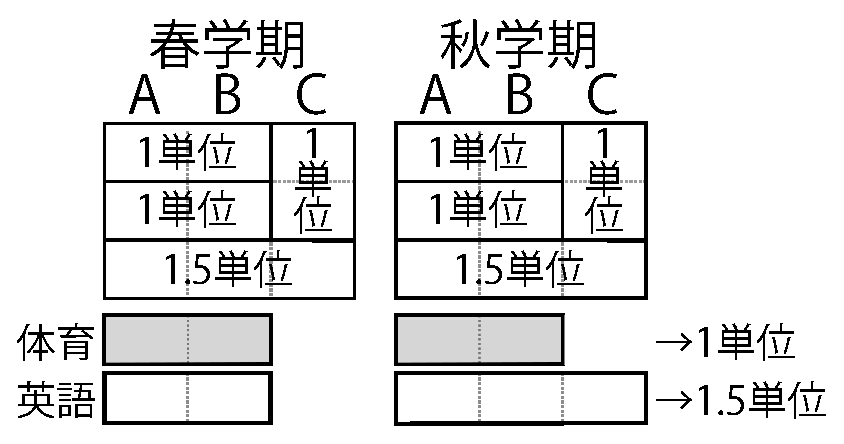
\includegraphics[width=0.45\textwidth,clip,keepaspectratio]{pic/01-introduction/tani.eps}
	\caption{2学期6モジュール制の単位}
\end{flushright}
\end{wrapfigure}
今年から\bold{2学期6モジュール制}になるため煩雑です。\note{面倒}
\\原則、\underline{\large\bf {\Large 1}コマ{\Large 1}モジュールで{\Large 0.5}単位}です。\\

\bparapara{例外}
\bold{実技科目}(実験など)は、通常の\bold{半分の単位数}\par
\footnote{例えば1年必修の情報科学基礎実験は1モジュールで4コマの授業を行う。
通常だと2単位だが、その半分の1単位になる。
単位制の根拠に由来し、実技科目は通常の科目より予習復習の時間が
少ないため単位時間分の学習量が少ないと考えるためである}
\bold{体育}は、4モジュール{\small (春AB,秋AB)}で\bold{1単位}\par
\bold{英語}\footnote{1年の英語は、基礎英語・総合英語・異文化と英語 の3つで、
1.5単位ずつで4.5単位分。今年度入学生から2年も英語が必修に。}
\bold{第二外国語}は、5モジュール{\footnotesize (春AB,秋ABC)}で\bold{1.5単位}


\subsection{履修制限について}
1年間で取得できる単位の最大は{\bf\Large 45単位}です
\footnote{この制限のことを「履修制限」や「キャップ」とかと呼ぶことが多い。}
。

学類長の許可が得られると1年間で\bold{55単位}まで取得できます。
履修要覧には「前年度の成績が6割以上がA」が条件とかいてあります
\footnote{履修要覧 情報学群履修細則 5条}。
1年は高校の成績を考慮すると聞きましたが、
臨機応変に対応することが多いようです。
昨年は50単位以上の場合は学類長との面談がありました。


\subsection{成績評価について}
成績評価はA+,A,B,C,D
\footnote{フレッシュマンセミナーなど成績評価ができない科目は、
成績評価がPとFになります。passとfail}となります。
A+,A,B,Cで単位が取れ、Dでは単位が取れません。
\\必修科目の単位が取れなかった場合、\bold{卒業できません}。
再履修してなんとしても取りましょう。

単位が取れた場合(A+,A,B,C)、再履修できません。その成績が残ります
\footnote{昨年までは良い成績が取れないと思った科目を故意にDか履修放棄にし、再履修して良い成績を残すという戦略があった。
\\しかし、この戦略ではGPAが下がるため陳腐化すると予想される\RA}
。


\subsection{GPA制度について}
\begin{wraptable}[7]{r}{0.4\textwidth}
\vspace{-10mm}
\begin{center}
\scalebox{1.1}{
\begin{tabular}{|c|c||c|c|}\hline
	成績評価&100点換算&単位&GPA\\\hline
	A+&90〜\hspace{1em}
	&\multirow{4}{*}{合格}&\cellcolor[gray]{1}4\\\cline{1-2}\cline{4-4}
	A &80〜89&&\cellcolor[gray]{0.96}3\\\cline{1-2}\cline{4-4}
	B &70〜79&&\cellcolor[gray]{0.93}2\\\cline{1-2}\cline{4-4}
	C &60〜69&&\cellcolor[gray]{0.88}1\\\hline
	D &\hspace{1em}〜60&\cellcolor[gray]{0.8}不合格  &\cellcolor[gray]{0.75}0\\\hline
\end{tabular}}
\end{center}
\end{wraptable}
単位は成績評価がA+,A,B,Cでも同じ単位数ですが、それぞれに重みを与えていこうとしたのが\bold{GPA制度}です
\footnote{型に言うと、単位はboolで、GPAはintのイメージ}。

GPAは大学院や就職するときに使われるます。通知表の内申点のようなものです。
主専攻を選択する場合にも同じようなものが利用されるようです。
\note{要出典}

GPAは履修した科目
\footnote{正確には学類が指定した科目区分で履修した科目、
coinsの場合は\bold{関連科目}はGPA算出にはいらない。詳しいことは後述}
の成績(左表)に単位数を掛けたものの\bold{平均}を取ります。

%\vspace{4mm}
\[\mbox{GPA}=\cfrac{\mbox{A${}^{+}$の単位数}\times 4 + \mbox{Aの単位数}\times 3 + \mbox{Bの単位数}\times 2 + \mbox{Cの単位数}}{\mbox{GPA対象科目の履修登録単位数}}\]
%\vspace{4mm}

Dを取り再履修した場合、分母が増えGPAは低くなります。
また、履修放棄
\footnote{履修申請したが履修申請期間後に履修登録を取り消すこと。}
した場合もD扱いとなりGPAは低くなります。

何でもかんでも履修して低い成績を取るとGPAは低くなってしまいます。
GPAを上げること\bold{だけ}考えると、
最低限の履修のみ申請し
テストは全力投球という形に必然的になってしまいます。

また、coinsでは後述の\bold{「関連科目」はGPA算出から除外}します。


\newpage
\vspace*{-8mm}
\section{履修計画をたてよう}


\subsection{科目区分について}
\begin{wrapfigure}[0]{r}{0.45\textwidth}
\begin{center}
\vspace{-15mm}
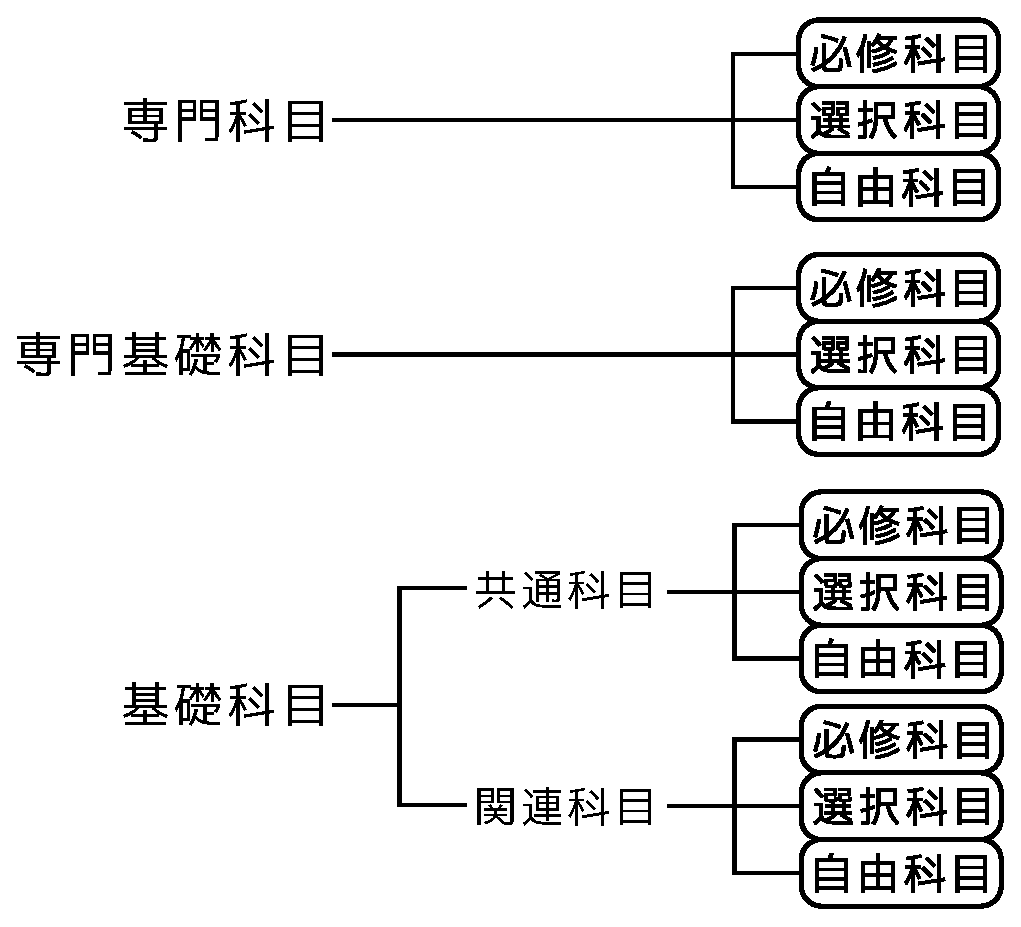
\includegraphics[width=0.4\textwidth]{pic/rishuyoran/kamokukubun.eps}
\end{center}
\end{wrapfigure}
\vspace{-2mm}
{専門科目}・{専門基礎科目}・{基礎科目}は、専門度による
\\区分です。単位換算の時は重要ですが、それ以外はあま
\\り違いありません。
\par 重要なのは\bold{必修科目}・\bold{選択科目}・\bold{自由科目}の区分です。

\bparapara{必修科目}
卒業までに\bold{取らないといけない}科目です。1年はこの
\\科目が多いです。なんとしてでも取りましょう。(2回目)
\bparapara{選択科目}
卒業までに指定した科目から一定単位数以上を取らないといけない区分です。
\\1年のうちは「力学」、「コンピュータ数学」、「情報社会と法制度
\footnote{情報\bold{学群}開設科目。専門選択}」
しかありません
\footnote{執筆現在、\bold{学群}開設科目(GAで始まる科目)の情報が少なかったため確認が必要}。

選択科目は2年から増えていきます。
\bparapara{自由科目}
好きな科目を履修して良い区分です。
また、余った選択科目を自由科目に変換することができます。
\footnote{履修申請するときに科目区分も指定するのだが、
履修期間内であれば変更はできる。
過ぎても3月まではtwinsで変更はできた(旧twinsの話)、
もしくは別途書類を作成、先生方のハンコを集めればできる}
総合大学なのでいろんな学類の科目が履修
\footnote{履修せず聴講という手もある。講義によるため要確認}
できます。
\bold{自由単位}と呼ばれます。

\subsection{卒業要件・進級要件について}
\vspace{-2mm}
これら要件は入学年度で決まっており、
原則卒業するまでその要件で過ごすことになります。

\bparapara{卒業要件}
卒業するために必要な単位の条件です。
これを満たしていないと卒業できません。
卒業要件は主専攻により多少異なりますが、
だいたい同じです。詳しいことは後述。

\bparapara{進級要件}
\bold{2年から3年}に進級するための条件です。
1年から2年へは特に条件はありません。

卒業要件で余裕のある履修計画を立てて実行すれば、
進級要件を読み込む必要はあまりありません。

入学してすぐ見るより最初の期末が終わったあたりに見ると
理解しやすいと思います。
単位を落とした場合・特殊な履修計画をした場合は、
よく確認することをおすすめします。

\subsection{卒業要件のみかた}
\vspace{-2mm}
これが履修要覧の\bold{情報学群履修細則}に載っている卒業要件です。

この表さえ理解しておけば、普通に卒業する分には十分です。
\bold{注釈が重要なのでちゃんと読みましょう。}

\newpage
\begin{figure}[H]
\begin{center}
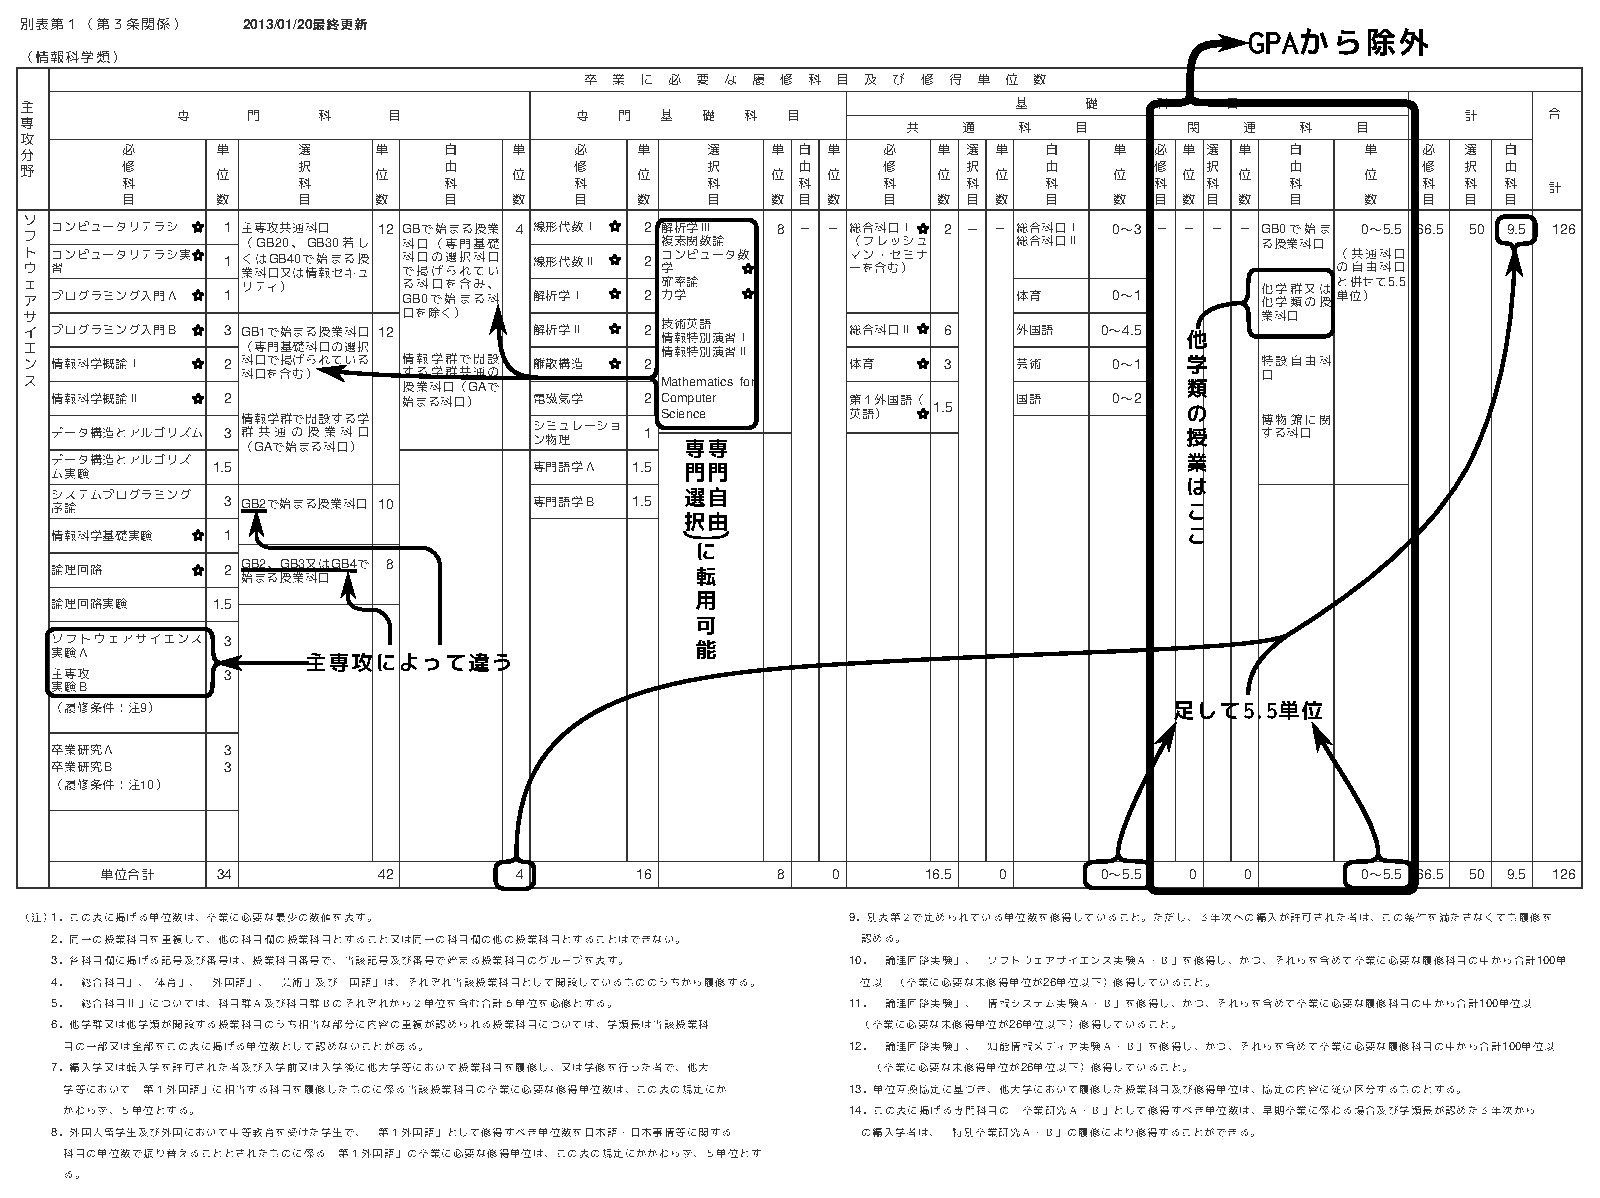
\includegraphics[height=0.72\textheight,angle=90]{pic/rishuyoran/req.eps}
\caption{平成25年度入学生 卒業要件}
\end{center}
\end{figure}
\newpage


\subsection{開設授業科目一覧のみかた}
だいたい見ればわかりますが、
開設授業科目一覧を左から説明していきます。
\vspace{-3mm}
\begin{table}[H]
\begin{tabular}{lcl}
$\rhd$科目番号&$\cdots$&twinsなどで履修登録するときに必要な番号\\
$\rhd$科目名・単位数&$\cdots$&科目の名前・単位の数\\
$\rhd$\bold{標準履修年次}&$\cdots$&履修が推奨される学年。
これより早く履修することも可能\\
$\rhd$実施学期・曜時限&$\cdots$&学期と時間、ダブルブッキングには気をつけて\\
$\rhd$\bold{教室}&$\cdots$&教室遠いと間に合わないことがある。3はエリア、Aは棟、209は教室である。\\
$\rhd$担当教員&$\cdots$&担当する先生の名前、相談することがあればシラバスに連絡先が書いてある\\
$\rhd$授業概要&$\cdots$&授業の概略、シラバスにはより詳細な授業計画が乗っている\\
$\rhd$\bold{備考}&$\cdots$&対象クラスや対象学類、履修する前に必要な科目などが乗っている。地味に重要
\end{tabular}
\end{table}
\vspace{-5mm}
\begin{figure}[H]
\begin{center}
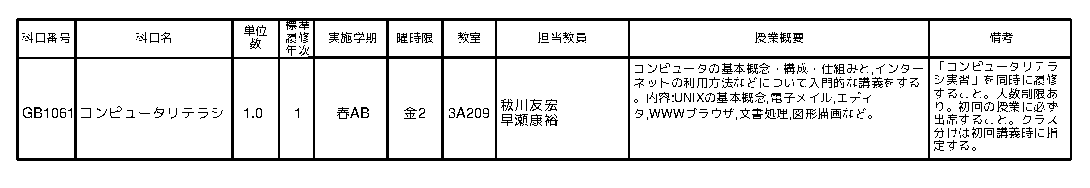
\includegraphics[width=0.8\textwidth,clip]{pic/kaisetu/online.eps}
\vspace{-2mm}
\caption{開設授業科目一覧より}
\end{center}
\end{figure}
\vspace{-8mm}

\subsection{時間割を組もう}
\bold{twins}
\footnote{筑波大学の履修申請システムのこと、
今年から一般公開され学外アクセスできるようになる
https://twins.tsukuba.ac.jp\note{たぶん合ってる}}
を開いて申請しながら履修計画を立てましょう。
履修期間中はいくらでも申請し直せますし、
時間割を見ながら作業できるので
ブッキングすることもありません。
本音を言うと、先生方がわかりやすくまとめてくださった時間割
\footnote{情報科学類シラバス参照。しかしこの時間割には
全学固定時間割を含んでいる。
教職科目や第2外国語など全員が取らなくても良い科目が
含まれているため注意}
通りに組めばほぼ完成してしまいます。
ですが、学年が上がると必修が少なくなり自分で立てる必要が出てくるので、
練習のつもりで1年からきちんと自分で立てましょう。

原則は\bold{\large 重要なものから入れる}です。

\begin{multicols}{2}
ちなみに、筑波大学の時間割は75分授業を採用しているので、1,2限が午前、残りが午後になっています。
休憩時間は15分です。


\vspace{0mm}
\begin{table}[H]
\begin{center}
\begin{tabular}{|r|l|}
\hline 1限 & {\textcolor{white}0}8:40〜{\textcolor{white}0}9:55 \\ 
\hline 2限 & 10:10〜11:25 \\ 
\hline 昼休み & 11:25〜12:15 \\ 
\hline 3限 & 12:15〜13:30 \\ 
\hline 4限 & 13:45〜15:00 \\ 
\hline 5限 & 15:15〜16:30 \\ 
\hline 6限 & 16:45〜18:00 \\ 
\hline 
\end{tabular} 
\end{center}
\end{table}
\end{multicols}


\bparapara{必修科目を入れる}
履修要覧の卒業要件に書いてある\bold{必修科目}を入れていきます。
この時、開設授業科目一覧の\bold{標準履修年次}も参照しながら、
自分の学年で受けるべきものを入れていきます。

\newpage
\bparapara{選択科目を入れる}
必修科目と同じように、標準履修年次を見ながら\bold{選択科目}入れていきます。余裕があれば入れて行きましょう。
専門基礎選択科目は専門選択・専門自由科目に転用できます。

\bparapara{自由科目を入れる}
\bold{自由科目}をいれます、
開設授業科目一覧を眺めて興味のある講義を
選んでください。

上の学年の必修や選択を先に取るという手もあります。
ですが、来年度講義が大幅改変があるため注意が必要です。

高校や中学校のように、時間割をすべて埋める必要はありません
\footnote{正確には履修制限があるためできない、
全て埋めなくてもGPAのことを考えると賢明ではない}。
空きコマにして課題をしたり、
バイトを入れたりすることもできます。
次の「空きコマの利用方法」で紹介します。

\vspace{5mm}

\bparapara{気をつけるべきこと}
入学したてのころはやる気と希望に満ちて
無理な履修計画を立てがちですが、
あとで絶望することがあります。
\bold{テストは時間割通りに行われる}ので、
一日中期末テストのようなことも起きます。
\vspace{2mm}

来年度、次の講義の内容が大幅改変するため、
今年度入学生が\bold{履修してはいけない}科目があります。
{\small\begin{itemize}
	\item データ構造とアルゴリズム
	\item データ構造とアルゴリズム実験
	\item 機械語序論
	\item ソフトウェア構成論
	\item ソフトウェアサイエンス概論2
	\item 情報システム概論2
	\item 知能情報メディア概論2
\end{itemize}}
いずれも標準履修年次の2年のものです。
逆をいえば、これらの科目以外なら履修してもよいのですが、
標準履修年次が2年のものなので慎重に決めてください。
\vspace{2mm}

また、これら以外にも\bold{45単位履修制限}や
\bold{GPA制度}があります。
このことも考えながら履修計画を立ててください。

twinsで申請するとき、\bold{科目区分}(専門必修科目や関連自由科目など)が
間違えないようにしましょう。
登録するときに最初から科目区分が入ってますが、
間違っていることもあるのできちんと確認しましょう。
万が一、履修申請期間後に気づいた場合、
書類を書いてスタンプラリー
\footnote{先生方にアポイントをとってハンコをもらうのを繰り返す}すれば変更できます。

あと、個人的な経験ですが、
昼食後の3時限目・体育のあとは絶望的に眠くなります。
自分も4月ぐらいに「そんなことはないだろう」
と甘く見ていました。
今はブラックコーヒーなりブルなりで気合入れてます。


\subsection{空きコマの利用方法}
比較的時間割の詰まってる1年でも空きコマは結構あります。
多くの人は課題をしたり、友達と駄弁ったり、昼食を取ったりしています。

空き時間の利用の仕方を私なりの視点で紹介します。
履修のことじゃないのでさくっと。

\newpage
\parapara{計算機室で過ごす}
coinsに24時間開かれている計算機室(通称:機室)。
計算機があるだけではなく、
課題をするために集まったりと
coinsの出会いの場のようになっています。
空調もあり、電源もありと素晴らしい環境です。
ちなみに、機室は飲食禁止です。
また、共有スペースなのであまり騒がないようにしましょう。

\parapara{ラウンジで過ごす}
\bold{情報科学類ラウンジ}(3C213\note{直した} 通称:ラウンジ)は
coinsだけでなくいろいろな人との出会いの場です。
昼食を食べてる人がいたり、勉強会をしたりします。
プロジェクターやホワイトボードがあるので
ちょっとした疑問を解決してもらったり、LTしたりできます。

\parapara{図書館で過ごす}
筑波大には、図書館が4つ
\footnote{中央図書館(第一エリア)・医学図書館(医学エリア)・体芸図書館(体芸エリア)・図情図書館(春日エリア)で4つ}
あります。
私はcoinsの本拠地3学に近い中央図書館をよく利用します。
自習室もあり電源もあります。プログラミング言語系の本は
図情図書館にも多くあるので見に行くと楽しいです。

\parapara{自室で過ごす}
筑波大学生は自宅が近いことが多いため、
普通の大学生だとできないことができます。
自室に帰って自由な時間を過ごせます。
一人暮らしだと買物洗濯家事なども自分でしないといけません。
ちなみに、私は一度家に帰るとおふとん重力圏から再脱出できず
苦労することが多いので帰らないことが多いです。

\vspace{5mm}
私はこんな感じですが、バイトを入れる人もいれば
サークルに行く人、実行委員会などの作業をする
ひともいます。
空きコマにはその人の個性が出ると思います。

うまく履修計画を立てて空きコマを有効利用していただけると幸いです。


\section{特殊な履修の仕方}
\subsection{教職課程について}
coinsでは中学の数学、高校の数学と情報の教職免許が取れます。
教職免許を取得するには、通常の学士課程とは別の\bold{教職課程}を取らないといけず、単位も別換算になります。

教職課程をとっている新歓委員に簡単な質問をしたものを載せておきます。

\parapara{Q1.現在coins12で教職課程を取ってる人の人数は何人ぐらいですか?(coins12は80名くらい)}
詳しい人数はわからないけれど5、6人です

\parapara{Q2.教職課程を取ることで大変なことはなんですか?}
まず単純に履修する科目が増えるので大変です。他の人よりもテストが多かったり、集中授業で土日がつぶれたりします。また周りに教職科目を履修する人がいないと気がついたら履修申請期間を過ぎているなんてこともあります。自分でしっかりと予定を見て計画を立てることも重要であり、大変です。

\parapara{Q3.教職課程を取る上で気をつけるべき点はなんですか?}
基本的に教職の情報は自分で集めることが必要です。情報科学類シラバスにも教職について書いてありますがあまりあてになりません。特に今年度からは二学期制が始まり、去年からの情報が当てにならないことも多いと思います。教職シラバスや支援室を積極的に使っていってください。

\parapara{Q4.教職課程を取ろうと志す新入生に一言おねがいします}
最初は楽でもどんどんつらくなっていくと思います。自分に負けずに頑張ってください。

\vspace{4mm}
教職課程は複雑なのでここでの詳しい説明は避けます。
履修要覧の
「教育職員免許等の取得に必要な科目の履修方法」
をみてください。
もしくは後述の履修相談会に参加してください。

\note{教職まんのokもらった}


\subsection{早期卒業について}
4年制大学を3年間で卒業できる制度で、
筑波大学のお墨付きがもらえるようなものです。
coinsのうちでも毎年1人いるかいないかだそうです。

詳しいことは履修要覧の情報学群履修細則に書いてあります。

2年終了時には85単位以上取得していなければならない上に、成績上位10\%に含まれなければならず、主専攻実験と卒業研究を同時にする強者でないとすることができません。

また、卒業時(3年)で卒業に必要な126単位を取得していないといけません。
卒業研究と主専攻実験が重いので1,2年のうちに他の科目を取っておく必要があり、
必然的に45単位履修制限を外さないと大変です。

私も目指してましたが、1年の期末試験のときに悟りました。非常にきついです。


\section{後記}
この冊子は今年から作り始めたました。

なぜかというと、
今年から2学期6モジュール制やGPA制度が導入され
「先輩の経験談」と違う部分が出てくることと、
私自身の反省があったからです。残りは趣味です。

そんなわけで、
冊子作成のノウハウが不足していたり、
そもそも何かけばいいかわからなかったり、
うまくまとめられた自信はありません。

「体育の服装は動ければいいからなんでもいいよ!
高校のジャージの人もいるよ!」のみたいな
大学にいないとわからない知識をもっと入れたかったのがですが、
尺の都合で切ってしまってちょっと後悔です。

\note{土日の履修の奴書くならここ}


\vspace{\fill}
\noindent\rule{\textwidth}{0.1mm}

4/13(土)の13時から1階の計算機室(3C113)で
\bold{履修相談会}をする予定です。

\noindent そこで、twinsを使いながら履修計画したり、
それぞれで個別に相談できたらなと思っています。

\noindent 履修に不安や疑問がある人はぜひぜひ、
twinsの申請するついでに$\cdots$みたい感じで十分です。

\noindent また、教職課程を目指す人がいれば個別に
説明できればいいなと考えています。

\hspace{\fill}\modtoday
\newpage
\thispagestyle{empty}
\vspace*{-1truein}%
\vspace*{-\topmargin}
\vspace*{-\headheight}
\vspace*{-\headsep}
\vspace*{-\topskip}
\vspace{14cm}
\begin{center}%
\noindent
\hspace*{-1in}
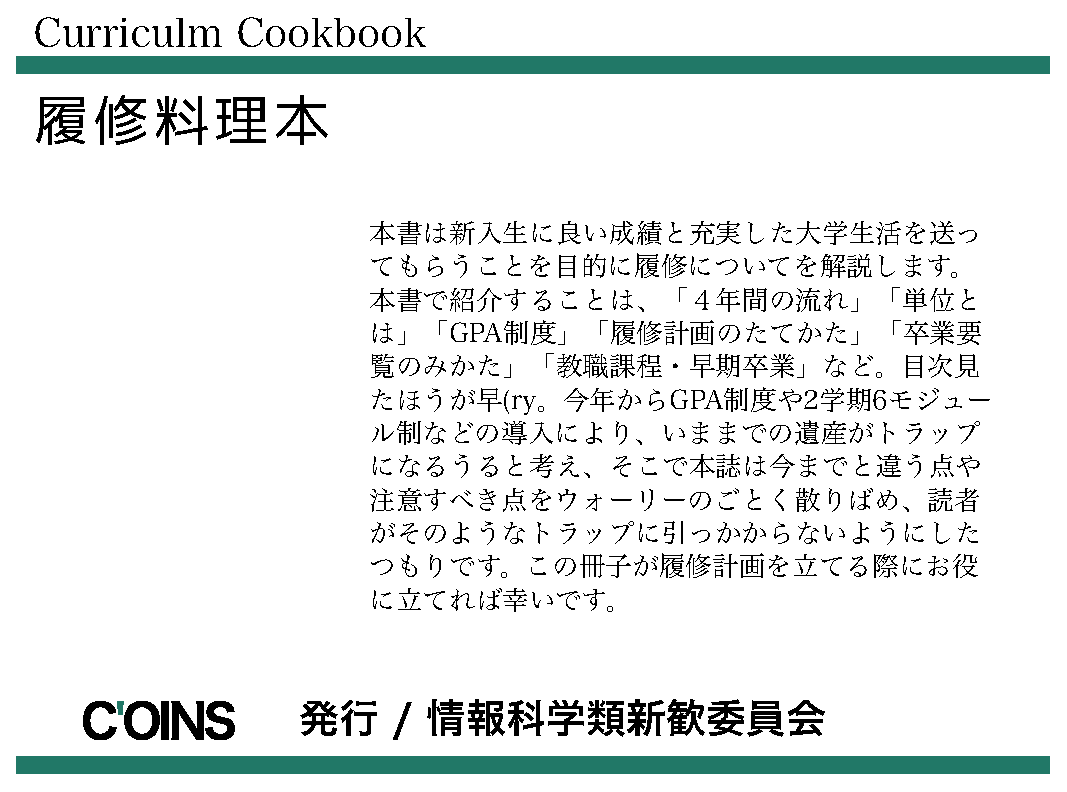
\includegraphics[width=1.1\fullwidth]{pic/hyousi/oreilly-back.eps}%
\hspace*{-1in}
\vspace*{-10cm}
\end{center}
\end{document}
